
\documentclass[titlepage,11pt,a4paper]{report}
%\usepackage[titlepage, fancysections]{polytechnique}
\usepackage[utf8]{inputenc} 
\usepackage[T1]{fontenc}
\usepackage[english]{babel}
\usepackage[toc,page]{appendix}
\usepackage{graphicx}
\usepackage[colorinlistoftodos]{todonotes}


\usepackage{todonotes}
\usepackage{caption}
\usepackage{subcaption}
\usepackage{float}
\usepackage{amsmath, amssymb, stmaryrd, bussproofs, amsthm}
\usepackage{tikz}
\usepackage{booktabs} 
\usepackage{subcaption}
\usepackage[nottoc,numbib]{tocbibind}
\usepackage{dashbox}
\usepackage{listings}
\usepackage{xcolor}
\lstset { %
	tabsize=2,
    language=C++,
    backgroundcolor=\color{black!5}, % set backgroundcolor
    basicstyle=\footnotesize,% basic font setting
}
\usepackage{tikz}
\usetikzlibrary{matrix, fit, calc}

\title{Denotational semantics for weak memory concurrency} 

\author{Anouk Paradis}

\date{July, 2018}



\theoremstyle{plain}
\newtheorem{theorem}{Theorem}[section]
\newtheorem{definition}{Definition}
\newtheorem{lemma}[theorem]{Lemma}
\newtheorem{proposition}[theorem]{Proposition}
\newtheorem{corollary}{Corollary}
\usepackage{afterpage}

\newcommand\ghost[1]{\dbox{\ensuremath{#1}}}
\newcommand\rPerm{R_{\lambda}^{EFC}(\text{bits})}
\newcommand\wPerm{W_{\lambda}^{EFC}(\text{bits})}
\newcommand\Uperm{\{\text{U}(\text { bits }, \mathcal{Q})\}}
\newcommand\emp{\mathrm{emp}}
\newcommand\ress[1]{resource(\texttt{bits})^{#1}} 
\newcommand\efcp[2]{\ghost{\lambda :(#1, #2)^{+}}}
\newcommand\efcm[2]{\ghost{\lambda :(#1, #2)^{-}}}
\newcommand\acqPerm{\operatorname{\mathsf{Acq}}(\ell, \mathcal{Q})}
\newcommand\acqPermp[1]{\operatorname{\mathsf{Acq}}(\ell, \mathcal{Q_{#1}})}
\newcommand\relPerm{\operatorname{\mathsf{Rel}}(\ell, \mathcal{Q})}
\newcommand\rmwPerm{\operatorname{\mathsf{RMWAcq}}(\ell, \mathcal{Q})}


\newcommand\consQ{\mathsf{Consumer}(\texttt{s.queue})}
\newcommand\prodQ{\mathsf{Producer}(\texttt{s.queue})}
\newcommand\sePred{\mathsf{SE}_\lambda(s)}


\newcommand\blankpage{%
    \null
    \thispagestyle{empty}%
    \addtocounter{page}{-1}%
    \newpage}

\begin{document}

\begin{titlepage}

\newcommand{\HRule}{\rule{\linewidth}{0.5mm}} % Defines a new command for the horizontal lines, change thickness here

\center % Center everything on the page
 
%----------------------------------------------------------------------------------------
%   HEADING SECTIONS
%----------------------------------------------------------------------------------------

%\textsc{\LARGE \'Ecole polytechnique}\\[1.5cm] % Name of your university/college
\textsc{\Large Research internship report}\\[0.5cm] % Major heading such as course name
\textsc{\Large Non confidential}\\[0.5cm] % Major heading such as course name
%\textsc{\large Minor Heading}\\[0.5cm] % Minor heading such as course title

%----------------------------------------------------------------------------------------
%   TITLE SECTION
%----------------------------------------------------------------------------------------

\HRule \\[0.4cm]
{ \huge \bfseries Verifying weak memory programs in the Viper ecosystem}\\[0.4cm] % Title of your document
\HRule \\[1.5cm]


 
%----------------------------------------------------------------------------------------
%   AUTHOR SECTION
%----------------------------------------------------------------------------------------

\begin{minipage}{0.4\textwidth}
\begin{flushleft} \large
\emph{Author:}\\
Anouk \textsc{Paradis} \\% Your name 
\small
Master of Computer Science\\
ETH
\end{flushleft}
\end{minipage}
~
\begin{minipage}{0.4\textwidth}
\begin{flushright} \large
\emph{Supervisors:} \\
Gaurav \textsc{Parthasarathy}\\ % Supervisor's Name
\small
PM Group\\
ETH\\
\textcolor{white}{lala}\\

Pr.~Alexander J.\textsc{Summers}\\ % Supervisor's Name
PM Group\\
ETH
\end{flushright}
\end{minipage}\\[2cm]

% If you don't want a supervisor, uncomment the two lines below and remove the section above
%\Large \emph{Author:}\\
%John \textsc{Smith}\\[3cm] % Your name

%----------------------------------------------------------------------------------------
%   DATE SECTION
%----------------------------------------------------------------------------------------

{\large \today}\\[2cm] % Date, change the \today to a set date if you want to be precise

%----------------------------------------------------------------------------------------
%   LOGO SECTION
%----------------------------------------------------------------------------------------

\includegraphics[width=3cm]{/home/anouk/2018/packageLatexPolytechnique/source/polytechnique-logovert.pdf}\\[1cm] % Include a department/university logo - this will require the graphicx package
 
%----------------------------------------------------------------------------------------

\vfill % Fill the rest of the page with whitespace

\afterpage{\blankpage}

\end{titlepage}


%\begin{abstract}
%		idkls;adkls;a
%\end{abstract}


\tableofcontents

\afterpage{\blankpage}

\chapter{Introduction}
Concurrent programs opened the way for tremendous gains of performance, and are now everywhere in our environment, from mobile phones to critical plants control. In spite of their ominpresence, their subtle functionning is still poorly understood, and there is not yet any fully satisfactory model for any widely used programming language, such as Java or C++. The need for such a model is patent : weak memory behaviors are not only non deterministic, that is to say they do not occur at every execution of a program, but they also depend on the processor used, and the optimizations the compiler performed. Bugs hence are not often exposed, and become difficult to detect, and even more difficult to track down. Furthermore, relying solely on testing, even extensive, and programmer's folklore about what should or should not happen means that the introduction of a new processor or compiler optimisation could uncover new behaviors in a program.

However, when designing such a model, one is faced with two opposing challenges. To allow for reasoning and verification of programs, the model should provide strong garanties about the permitted behaviors. Alas, it should also allow for performance, and hence for the counterintuitive relaxed behaviors hardware and compiler optimisations may introduce.

On top of those two antagonistic intents, such a model should have the following characteristics to be fully usable. First, as most programs today are not built as one monolithic block of code, but rather as mutliple interconnected blocks, that might even be running on different processors, the model should aim for compositionality\cite{BattyRoyalSoc}. That is to say it should allow reasoning on the whole program to be the composition of reasoning on each block. Second, it should be usable by programmers. This can be done through different means. First the model should aim to be as simple and intuitive as possible. A simulator of the model on simple executions, as was provided by \cite{BOSSW11} for the C++11 standard is also of great help. Such a simulation is not always yet possible, for instance for \cite{KHLVD17}, as it requires quantification over all future possible memory states. Another important way to improve usability of the model is the so-called DRF-SC theorem. This theorem relies on the notion of sequential consistency \cite{LamportSC} : the behavior of a program is sequentially consistent if it can be explained by a simple interleaving of the different threads actions. The DRF-SC theorem is then stated as : if a program is data race free for any sequentially consistent execution, then all its executions (even the relaxed ones) do not exhibit any behavior that is not exhibited by a sequentially consistent execution. It is extremely usefull, as it allows programmers to completely ignore weak memory behaviors when building a program with a strong lock discipline. Hence only programs with a strong need of performance need to deal with weak memory behaviors.


\paragraph{Note :} The topic of my internship was initially "An RCU specification in fixed C++ concurrency". However it changed to focus on working on the memory model itself, as it was not yet usable for an application to the RCU algorithm.

\paragraph{Contributions}
When I began my internship, a simple language and its semantics had already been defined, as well as a model that could deal with dependancies. A more complicated model had also been defined to deal with fences and ordering. However, it did not work properly for many widely accepted small programs.
At the end of my four months internship, we were able to develop a different model, using the idea of dependency developped in the first model, that could also deal with fences and atomics, as they are defined in the C++ language. It behaves properly on the litmus tests demonstrating many weak behaviors introduced by Power Multiprocessors, as presented by \cite{powerMultiProc}. We also defined a similar model for non atomics and locks and were able to prove that the DRF-SC theorem holds for this simplified model.
Finally, these models are built compositionaly, that is to say we have a representation even of incomplete programs, and can compose them together. This could allow for reasoning on a subpart of a program, and using those results when reasoning on a whole program.


\chapter{Background and related work}
djksljflkdsjfldks

fetch and add  + cas - false rules (fig 3 et 4 de gaurav p/13)

\chapter{Ease of use limitations of the EFC ghost location and tokens}
\label{sec1}
In this chapter, we will use the Folly library reader writer lock \cite{follyRW} to explicit some limitations of the EFC monoid defined in \cite{gaurav} and the token-based reasoning developed in \cite{pascal}. While, as we will see, those limitations can easily be overcome using some simple tricks, they make reasoning less intuitive, and those tools harder to use.

\section{The Folly reader-writer spinlock}
The Folly reader-writer lock is used to allow multiple threads to access concurrently a shared resource \emph{res}, with either reader or writer privilege. This lock allows multiple reader threads to access \emph{res} concurrently, but makes sure that if a thread has write access, all other threads are forbidden from reading or writing to it. The (simplified) implementation of this lock is shown in Figure~\ref{fig:follyRWL}. This implementation is taken from \cite{gaurav}.

\begin{figure}
	\begin{lstlisting}
	bool  try_lock_shared ()
{
	v0:=fetch_and_add_acq(bits,4)//RMW1
	if(lsb(v0) == 1) {
		v1:=fetch_and_add_rel(bits,−4)//RMW2
		res :=  false
	}
	else {
		res := true
	}
	return  res
}

void  unlock_shared () {
	x:=fetch_and_add_rel(bits,−4)
}

bool  try_lock () {
	v:=CAS_rel_acq(bits,0,1)
	return (v == 0)
}

void  unlock(bool  getRead) {
	x:=fetch_and_and_rel(bits,∼1)
}

void  unlock_and_lock_shared () {
	x:=fetch_and_add_acq(bits,4)//RMW1
	unlock(true)
}
	\end{lstlisting}
\caption{Folly RW lock implementation (from \cite{gaurav})}
		\label{fig:follyRWL}
\end{figure}

The idea of the implementation is quite simple. It uses an atomic location \emph{bits}. The least significant bit of \emph{bits} (which we will denote as \emph{lsb(bits)})indicates whether or not there is currently a thread with write access, while \emph{bits / 4} indicates the number of threads currently having or attempting to have a read access. When a thread wanting a read access to \emph{res} calls the function \texttt{try\_lock\_shared()}, it first increments \emph{bits} by 4. Then it checks for the value \emph{lsb(bits)} had when it was incremented by 4. If it is null, then there is currently no writer thread. The call to \texttt{try\_lock\_shared} succeeded, and the calling thread got read access. If it is not null, the thread decrements \emph{bits} by 4 and the call failed: no access is gained. To release a reader lock, a thread simply decrements the \emph{bits} variable by 4, using the \texttt{unlock\_shared} function. To get a write-lock, a thread calls \texttt{try\_lock}, which simply atomically checks if \emph{bits} is 0 (that is to say there is no reader thread or thread currently attempting to get read access), and if so changes it to 1. Finally, to release a writer-lock, \emph{lsb(bits)} is simply set to 0.

\section{Proof using the EFC permission structure}
As explained in more detail in Chapter~\ref{ch:background}, the EFC permission structure is based on the idea of giving entities, containing some amount of permission and a token, to each thread that asks for it. We then record the number of tokens, and the total amount of permission that were distributed, to be able to track if full permission is available or not. 

Hence, when trying to prove this implementation to be correct using the EFC permission structure, the first idea that comes to mind is to use only one ghost state in the invariant, quantifying how many permissions, and which amount of permission were given away. This leads to the following invariant:

$$\begin{aligned} \mathcal{Q}^{EFC}(v) :=& \operatorname{let} n=\left\lfloor\frac{v}{4}\right\rfloor + lsb(v), w=\operatorname{lsb}(v), \text { in } \\ & \exists s \in \mathbb{Q} \cap[0,1] \cdot v \geq 0 \wedge (w=1 \Leftrightarrow s=1) \wedge \\ & resource(\mathrm{bits})^{1-s} * \ghost{\lambda :(n, s)^{-}}
\end{aligned} $$

while the read and write permission are represented by:
$$\rPerm = \exists q \in (0, 1].\ress{q}* \ghost{\lambda : (1, q)^+}$$

$$\wPerm = \ress{1} * \ghost{\lambda:(1, 1)^+}$$

Here a read permission is tracked with a token and some non null amount of permission $\ghost{\lambda :(1, q)^+}$, while a write permission corresponds to the full permission 1: $\ghost{\lambda:(1, 1)^+}$. The source $\ghost{\lambda :(n, s)^{-}}$ in the invariant tracks the number $n$ of tokens that were given away, as well as the amount of permission $s$ that was given along. Finally, in the \texttt{try\_lock\_shared} function, a thread may increment the location \emph{bits} without actually gaining any permission, if there is already a writer thread along. In this case, the thread temporarily gets an empty token, with no permission $\ghost{\lambda:(1, 0)^+}$.  We show in Figure~\ref{fig:specRWFolly} the function specifications we would like to prove. 

Note that here the tokens represented by the ghost location do not hold any permission by themselves, they are simply used to track the permission that is actually transmitted through $\ress{q}$.

\begin{figure}
		$$\Uperm \texttt{bool try\_lock\_shared()}\{y. (y ? \rPerm : \emp)\}$$
\[
\left\{\begin{array}{l}\Uperm* \\ {\rPerm}\end{array}\right\}
\texttt{void unlock\_shared()} \{\emp\} \]


$$\{\Uperm\}\texttt{bool try\_lock()} \{y. (y ? \wPerm : \Uperm)\}$$


\[
\left\{\begin{array}{l}\Uperm* \\ \wPerm* \\ (\texttt{getRead} ? \\ \ghost{\lambda: (1, 0)^+} : \\ \emp) \end{array}\right\}
\texttt{void unlock(bool getRead)}
\left\{\begin{array}{l}(\texttt{getRead} ? \\ \rPerm : \emp) \end{array}\right\} \]

\[
\left\{\begin{array}{l}\Uperm* \\ \wPerm* \end{array}\right\}
\texttt{void unlock\_and\_lock()}
\{\rPerm\} \]
\caption{Specifications of the lock functions}
\label{fig:specRWFolly}
\end{figure}

While this invariant and specifications seem quite straightforward, they are not sufficient to prove correctness of the \texttt{unlock\_shared} function. Let us go through the proof.

We use the fetch-and-add rule shown in Figure~7 of \cite{fsl}, using $\mathcal{P}_{\text{send}} = \rPerm$ and $\mathcal{P}_{\text{keep}} = \emp$. It is hence sufficient to show that for all values  $v \geq 0$, we have that 

\[
\begin{array}{l}
\{\Uperm * \rPerm\} \\
\texttt{CAS}_{\text{rel}}(\texttt{bits}, v, v - 4) \\
\{y. (y = v \land \emp) \lor (y \neq v \land \Uperm * \rPerm)\}
\end{array}\]

To do so, we use disjunction.
If $v < 4$ and $\texttt{lsb}(v) = 0$, we have that $\mathcal{Q}(v) \Rightarrow \efcm{0}{0} * \text{true}$ (we here use that $(0, x)$ is in the domain of the EFC permission structure if and only if $x = 0$). We hence have that $\mathcal{Q}(v) * \efcp{1}{0} \Rightarrow \text{false}$, as $\efcp{1}{0} \oplus \efcm{0}{0}$ is undefined. The \textsc{cas}-$\bot$ rule from \cite{fsl} then allows us to conclude this case.

The second case is $v < 4$ and $\texttt{lsb}(v) = 1$. In this case we have that $\mathcal{Q}(v) \Rightarrow \efcm{1}{1}$. We hence have again that  $\mathcal{Q}(v) * \efcp{1}{0} \Rightarrow \text{false}$, as $\efcp{1}{0} \oplus \efcm{1}{1}$ is undefined. We then use the \textsc{cas}-$\bot$ rule again.

The proof then fails for the case $v \ge 4$ and $\texttt{lsb}(v) = 1$. In this case, we would like to use again the \textsc{cas}-$\bot$ rule: in our implementation, this can never happen, as we cannot at the same time have given a write permission (as denoted by $\texttt{lsb}(v) = 1$) and a read permission (currently owned by the thread calling \texttt{unlock\_shared}). However, the invariant fails to capture this idea. The only information we can get from it here is that the amount of permission that was given away in total is $1$. For instance an invariant containing the ghost location $\ghost{\lambda:(3, 1)^-}$ could denote either that 3 readers each got permission 1/3 to the resource, or 1 writer got full permission, and two threads are trying to get reader access (and are currently running the \texttt{try\_lock\_shared} function). We could not express using only one ghost location that the first case cannot happen.

While this example shows that the EFC permission structure is a bit less expressive than we can think it to be at first sight, this proof can easily be made to work using one extra ghost location, as is done in \cite{gaurav}. This extra ghost location captures exactly the information we showed was lacking before: is there currently a thread owning write permission?

It is interesting to note that this problem is not encountered in the Rust Atomic Reference Counter proof using an EFC ghost state developed in \cite{gaurav}. This is simply because in this case, we only ever give away read accesses. It can hence be hardcoded in the invariant that the amount of permission given away is always strictly less than 1.



\section{Proof using token-based reasoning}
We saw in the previous section how the EFC permission structure is weaker in practice than what our intuition dictates. While this limitation can easilly be overcome, it is at the price of slightly less intuitive proofs. We will see here that the token-based reasoning developped in \cite{pascal} is itself weaker than the EFC permission structure it was based on.

If we were to straightforwardly translate the proof developped in the previous section using the tokens defined in \cite{pascal}, we would get the invariant and read and write permissions shown in Figure~\ref{fig:invToksRWFolly}.

\begin{figure}
$$\begin{aligned} \mathcal{Q}^{EFC}(v) :=& \operatorname{let} n=\left\lfloor\frac{v}{4}\right\rfloor + lsb(v), w=\operatorname{lsb}(v), \text { in } \\ & v \geq 0 \wedge (w = 1 ? \texttt{Src}(res, n, write) : \texttt{Src}(res, n, read))
\end{aligned} $$

$$\rPerm = \texttt{Tok}(res, 1, read)$$

$$\wPerm = \texttt{Tok}(res, 1, write)$$
		\caption{Simple invariant and Read-Write permissions for the Folly Reader-Writer Spinlock}
		\label{fig:invToksRWFolly}
\end{figure}

Now, in the \texttt{unlock\_shared} function, we would like to prove that we cannot read $v < 4$ from the location \texttt{bits}. Here we cannot do it, as the token we own is not incompatible with the location invariant. Reading $v < 4$ and $lsb(v) = 1$ from \texttt{bits} yields $\texttt{Src}(res, 1, write)$. Using the \textsc{any-src-read-tok}, we could then combine the source with our read token to get $\texttt{Src}(res, 0, read)$, which using the \textsc{all-tokens-a} yields $\texttt{Src}(res, 0, write)$. We could not reach any contradiction here.

This is because the tokens allow for "downgrading" of a token, from write to read permission. Hence is could happen that a threads gets write permission, downgrades it to read permission, then gives back this permission. The source then has to be able to reconstruct from the number of tokens it has wether or not it now owns full permission or not. This could not happen using the EFC ghost state directly as such a downgrading of tokens is not possible: the amount of permission $q$ contained in a ghost location $\ghost{\lambda : (1, q)}$ cannot be made lower without further dividing the token.

We here see that the proof fails earlier than when using the EFC permission structure, showing a small difference between the two reasonings. This can again be easilly fixed, by making the proof a little less straightforward. We can for instance use the idea developped in \cite{pascal} for the Rust Atomic Reference Counter proof: defining a different amount of tokens for read an write permissions. This outcome can then be forbidden. By giving 3 tokens for read permission and 2 for write, we would reach a contradiction by trying to combine  $\texttt{Src}(res, 2, write)$ and $\texttt{Tok}(res, 3, read)$, using rule \textsc{too-many-tokens}. This trick allows us to get as far in the proof as we did using the EFC ghost location, but we then get stuck in the next step: proving that $v \geq 4$ and $lsb(v) = 1$ is not possible. This is what we would expect: the tokens are not more powerful than the EFC ghost location.


\chapter{Limitations of FSL++}
In the previous section, we showed some limitations of the EFC permission structure and the token-based reasoning. However, those limitations could be overcome, though they made proofs less intuitive and hence harder to write. In this section, we will develop on some limitations of FSL++. Those limitations seem more fundamental, as we could not find ways to overcome them, and at least one would require an extension to the FSL++ logic. We will develop those limitations using two examples, from the glibc and Folly libraries.

\section{glibc Reader-Writer Lock}
We will first focus on the glibc Reader-Writer lock \cite{glibcRW}. As we will see in Section~\ref{subsec:glibcRWPb}, it cannot be proven in FSL++ for a deceptively simple reason. We will still describe it in details, as its synchronisation mechanism is quite interesting, and shows how a slightly different implementation can make for different (or impossible in this case) proofs.

\subsection{Implementation}
The implementation of this lock is shown in Appendix~\ref{app:glibc}. This implementation was heavily simplified from the original one. In particular, futexes (special variables used to wake-up a thread when an event occurs) which where used to prevent extra spining where removed. While they are important to make the code more efficient, they are not part of the synchronization mechanisms used to ensure correctness of this lock.

\begin{figure}
		\begin{center}
		\includegraphics[width=\linewidth]{schemaglibc.png}
		%\caption{glibc reader-writer lock}
		\end{center}
		\caption{glibc reader-writer lock}
		\label{schemaglibc}
\end{figure}

Just as the Folly reader-writer lock, this lock offers four main functions: \texttt{readLock} (equivalent of \texttt{lock\_shared}), \texttt{readUnlock} (\texttt{unlock\_shared}), \texttt{writeLock} (\texttt{lock}) and \texttt{writeUnlock} (\texttt{unlock}).

This implementation uses a single atomic location \texttt{\_\_readers}. This location is used as shown in Figure~\ref{schemaglibc}. The least significant bit is used to denote if the lock is in read or write phase. As can be expected, if it is in read phase, only reader access can be granted, while if it is in write phase, only writer access can be granted. The second least significant bit tells wether or not there is currently a thread asking for or having write access. Finally, \texttt{\_\_readers} $/ 8$ gives us the number of threads currently owning reader access or requesting it. For easier reading, we use the following denotation for the value of \texttt{readers\_\_}: $\mathtt{readers\_\_} / 8 | lsb(\mathtt{readers\_\_ }/ 2) | lsb(\mathtt{readers\_\_})$. For instance, $2|1|1$ corresponds to \texttt{readers\_\_} $=19$, which means the lock is currently in write phase, and that one thread owns a write access, while two threads are requesting a read access. If it were to contain $2 | 0 | 1$, it means it is still in write mode, but no thread owns write access to it. The implementation makes sure that in this case one of the threads requesting read access will change the least significatn bit to $0$, allowing for read access.

Each of the function then uses appropriate synchronization mechanisms to ensure the value of \texttt{\_\_readers} accurately reflects the permissions threads hold to the protected location, as well as proper synchronization when taking or releasing the lock. A more detailed explanation of the lock implementation can be found in the Appendix~\ref{app:glibc}. The synchronization mechanisms are quite complex, and not necessary to understand the following.

We will here only focus on a further simplification of the \texttt{readerLock} function which is sufficient to show the different mechanisms we are interested in. 
%We simply remove loops and replace them with \texttt{if} statements. Note that note only the call to lock can now fail, but it may also put the lock in an inconsistent state (as it may increment the number of readers, and never decrement it). However, we are here only interested in successfull executions of this simplification. 
This simple code is shown in Figure~\ref{fig:codeglibc}.

\begin{figure}
		\begin{lstlisting}
Constants:
WRLOCKED = 2
WRPHASE = 1

int readLock(){
	int r = fetchAndAdd_Acq(__readers, 8) + 8
	if(r & WRPHASE == 0)
		return 0
	while(r & WRPHASE != 0 && r & WRLOCKED == 0){...}

	while(Load_Acq(__readers) & WRPHASE == 1){;}
}

	\end{lstlisting}
	\caption{\texttt{readLock function}}
	\label{fig:codeglibc}
\end{figure}
In the rest of this section, we will only use two executions scenarios to support our reasoning. They are shown in Figure~\ref{fig:scen1} and Figure~\ref{fig:scen2}. The first one is the most straightforward: there is only one thread trying to get the lock. It calls \texttt{readLock()}. The \texttt{fetchAndAdd} occurs, increasing the number of potential reader threads to 1. We then check if the least significant bit (corresponding to \texttt{WRITEPHASE}) is set to 0. As it is the case, the function returns: the thread now has a read lock. In the second scenario, Thread 1 holds a write lock when Thread 2 calls the \texttt{readLock} function. Hence after the \texttt{fetchAndAdd}, neither the \texttt{if} condition nor the following \texttt{while} condition succeed. Thread 1 then releases the lock. The condition of the final \texttt{while} is then satisfied. The function returns and Thread 2 now holds a read lock.

We see here that the calling thread can get read access to the resource in two distinct points \footnote{There is actually a third one in the elided code, but it is not relevant to our discussion here}. This is quite different from the Folly reader-writer spinlock implementation, where the access was granted by the \texttt{fetchAndAdd} operation only. If the lock was already taken, the function would cancel this add (by substracting the same value), and fail. We will see now how this proves to be a problem when formalizing this lock in FSL++.


\begin{figure}
\begin{tabular}{c||c}
	\texttt{\_\_readers} & Thread 1\\
	0 | 0 | 0 & \\
	 &   \texttt{fetchAndAdd\_(\_\_readers)} \\
	1 | 0 | 0 & \\
	 & \texttt{if(r \& WRPHASE == 0) } \\
	& \texttt{return 0 } \\
	&  Read lock succeeds!
\end{tabular}

		\caption{First \texttt{readLock()} execution scenario}
		\label{fig:scen1}
		%\caption{First \texttt{readLock()} execution scenario}
\end{figure}
\begin{figure}
\begin{tabular}{c||c|c}
	\texttt{\_\_readers} & Thread 1 & Thread 2 \\
	0 | 0 | 0 & & \\
	 & \texttt{writeLock()} & \\
	0 | 1 | 1 &   & \\
	 &   & \texttt{fetchAndAdd\_(\_\_readers)} \\
	1 | 1 | 1 & & \\
		& & \texttt{if(r \& WRPHASE == 0) ...} \\
		& & \texttt{while(r \& WRPHASE != 0 ...} \\
	 & \texttt{writeUnlock()} & \\
		1 | 0 | 0 & & \\
		& & \texttt{Load\_Acq(\_\_readers) \& WRPHASE} \\
		& & Read lock succeeds!
\end{tabular}

		\caption{Second \texttt{readLock()} execution scenario}
		\label{fig:scen2}
		%\caption{Second \texttt{readLock()} execution scenario}
\end{figure}


		\subsection{Read-Modify-Write and Load}
	\label{subsec:glibcRWPb}
As we saw in the two executions scenarii described above, read permission can be given either by a fetch-and-add, or by a subsequent load. However, when looking into the proof rules of FSL++, none of them allow for gaining resources from a single atomic location both using a Load and a fetch-and-add. When looking further into it becomes quite clear why such a rule would be quite difficult to implement.

In FSL++, atomic locations are used to transfer ownership (here to the resources protected by the lock) between threads. It does so by using a location invariant $\mathcal{Q}$ which for each value $v$ gives the ownership corresponding to this value. Then when writing value $v$ to the atomic location, a thread has to give up the assertion $\mathcal{Q}(v)$, and when reading value $v$, a thread gains this assertion. However this simplistic idea is not sufficient: it could happen that Thread 1 writes $v$, giving up $\mathcal{Q}(v)$, then Thread 2, reads $v$, gaining $\mathcal{Q}(v)$, then Thread 3 reads as well $v$, gaining $\mathcal{Q}(v)$. Here, the assertion $\mathcal{Q}(v)$ has been duplicated, which is clearly unsound \footnote{For instance if $\mathcal{Q}(v) = \ress{1}$, this would lead to total permission access to a location striclty greater than 1.}. To forbid this outcome, FSL++ introduces the assertions $\acqPerm$ and $\relPerm$. When a new variable is created, the corresponding permissions $\{\acqPerm * \relPerm\}$ are created. $\relPerm$ can then be freely duplicated, whereas the $\acqPerm$ can only be transmitted, making sure only one thread is allowed to get ownership from the location (all threads can read from the location, but they will get no ownership from it). 

Now for read-modify-write operations, that is to say operations that read and write atomically to a variable, the situation is different. As the value of the variable is read and changed in one atomic operation, the duplicating problem does not occur anymore. If thread 1 does a fetch-and-add and reads value $v$, it gets $\mathcal{Q}(v)$, and gives $\mathcal{Q}(v + 1)$. Hence if another thread then does another fetch-and-add there is no risk of inadvertently getting twice the same permission. Hence we can be more permissive heere, allowing multiple threads to perform read-modify-writes to the same location, and all gaining ownership. To allow for this, when a new variable is created, FSL++ offers a choice between $\relPerm * \acqPerm$ or $\relPerm * \rmwPerm$. The latter is then freely duplicable and can be transmitted to all threads requiring it. There is howver no rule that would allow to have both $\operatorname{\mathsf{Acq}}(\ell, \mathcal{Q}_1)$and $\operatorname{\mathsf{RMWAcq}}(\ell, \mathcal{Q}_2)$ for the same location, with $\mathcal{Q}_1$ not empty.

A new logic rule that would allow for this would be difficult to design, as it would have to take into account the duplicability of $\rmwPerm$ and non duplicability of $\acqPerm$.

	\subsection{Separation of tokens and permission}
We saw in the previous section how FSL++ rules do not allow for a proof of the glibc reader-writer lock. Another interesting point of this lock when thinking in terms of the EFC permission structure, is that it separates tokens from permission. In the second scenario Figure~\ref{fig:scen2}, thread 2 increments the number of readers with the fetch-and-add, but only gets permission with the load in the second while. This would hence make counting the number of permissions given away (as recorded by \texttt{\_\_readers / 8}) difficult to link with the amount of permission given (done in the load here).

\section{Folly One Producer One Consumer Queue}
\label{sec:2b}
We saw in the previous section that we could not use FSL++ to prove strong results about the glibc reader-writer lock, because it lacked support for both read modify writes and loads to the same variable. We will now focus on a different example, using only store/load, to avoid encountering this shortcoming again.

This new example is the Folly ProducerConsumerQueue \cite{queue}, a concurrent fixed size queue. It allows for exactly one producer thread, and one consumer thread. The queue is implemented using a circular buffer, as well as release stores and acquire loads for synchronization. The full code, including some extra functions that we will not discuss can be found in Appendix~\ref{app:queue}. We will here use the simplification of the code shown in Figure~\ref{fig:queueCyclic}.

An object \texttt{Queue} contains four fields: its size, an array \texttt{records} of size \texttt{size\_}, and two atomic indices \texttt{readIndex, writeIndex}. When creating the object, both indices are set to $0$. The queue offers two main functions: \texttt{write} which takes an argument and adds it to the queue if it is not full, and \texttt{read} which returns the last element if the queue is not empty. 

Note here that in spite of its name, the read function requires full ownership to the array slot it is reading, as it deletes it when returning it. This means that the producer and consumer threads need to transfer full ownership between one another during those function calls.

\begin{figure}
\begin{lstlisting}
bool write(toWrite){
	int curWrite = load_rlx(writeIndex)
	int nextWrite = (curWrite + 1) % size_
	int curRead = load_acq(readIndex)
	if(nextWrite != curRead){
		records[curWrite] = toWrite
		store_rel(writeIndex, nextWrite)
		return true
	}
	return false
}
bool read(&valRead){
	int curRead = load_rlx(readIndex)
	int nextRead = (curRead + 1) % size_
	int curWrite = load_acq(writeIndex)
	if(curRead == curWrite)
		return false
	valRead = records[curRead]
	delete records[curRead]
	store_rel(readIndex, nextRead)
	return true
}

\end{lstlisting}
		\caption{Simplified code for the Folly one producer one consumer queue}
		\label{fig:queueCyclic}
\end{figure}

This code is quite simple. Let us focus on the \texttt{read} function in more detail. This function first reads the current read index. Note that this read is relaxed. It is used here only to have a nicer interface for the function: as there is only one consumer thread, this thread could remember the \texttt{readIndex} value from one call to another, and pass it as an argument to the function, without fundamentally changing the function. We then compute the position of the next slot in the array (which we use as a circular buffer hence the need for \%). The first synchronization then comes in: the value of \texttt{writeIndex} is read with an \texttt{acquire} synchronization. This synchronization ensures that all reads or writes that come after will not be re-ordered before. We then check whether the queue is empty. If not, we store the current record in the reference that was passed as argument to the function, then delete the record. Finally, we use a release store to update the value of \texttt{readIndex}.

\begin{figure}
		\begin{center}
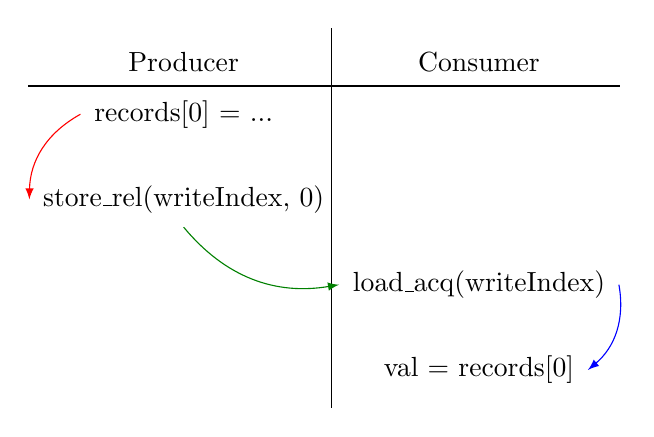
\begin{tikzpicture}%
  \node[%
  matrix of nodes,%
  inner xsep=0pt,% <- code added
  every node/.append style={%
    draw=white,
    inner xsep=5pt,
    inner ysep=5pt,
    outer sep=0pt,
  },
  row sep=0pt,
  column sep=0pt
  ] (M) {
    Producer & Consumer \\
	records[0] = ... & {} \\
	{} & {}\\
	store\_rel(writeIndex, 0) & {} \\
	{} & {}\\
	{} & load\_acq(writeIndex) \\
	{} & {}\\
	{} & val = records[0] \\
  };
% horizontal lines
  \draw[black]({$(M-1-1)!.5!(M-1-2)$} |- M.north) -- ({$(M-1-1)!.5!(M-1-2)$} |- M.south);
  %\draw[orange!80!black]({$(M-1-2)!.5!(M-1-3)$} |- M.north) --({$(M-1-2)!.5!(M-1-3)$} |- M.south);
% vertical lines
    \node[fit=(M-2-1) (M-2-2),inner sep=0pt] (R2) {};
    \draw[black] (R2.north -| M.west) -- (R2.north -| M.east);
%hb
		\draw[red,->,>=latex](M-2-1.west) to[bend right] (M-4-1.west);
		\draw[green!50!black,->,>=latex](M-4-1.south) to[bend right] (M-6-2.west);
		\draw[blue,->,>=latex](M-6-2.east) to[bend left] (M-8-2.east);
\end{tikzpicture}
\end{center}
%\label{fig:synchQueue}
\caption{Synchronization in the Folly one producer one consumer queue}

\label{fig:synchQueue}
\end{figure}


To better explain the synchronization ensuring that there is no data race on \texttt{records}, we focus on a simple scenario: we start from an empty queue, the producer thread then stores a value in \texttt{records}, and the consumer thread then reads it. Part of this scenario is shown in Figure~\ref{fig:synchQueue}. The release store to \texttt{writeIndex} ensures that any memory operation happening before it will be visible to other threads when they see the value released. In particular, any thread reading the new value of \texttt{writeIndex} will have the proper value stored in \texttt{records[0]}. This is materialized by the red arrow. Then the acquire load ensures that any memory operation after it will not be re-ordered. In particular, reading in \texttt{records[0]} will happen after this value was read, as shown by the blue arrow. Finally, as in this scenario the load acquire reads the value from the previous release store, we have an ordering between the two shown by the green arrow. There is hence a proper ordering between the write access to \texttt{records[0]} by the producer thread and the read access to it by the reader thread: data races are avoided.

\subsection{Re-using values for location invariants}
We saw in the previous section about the glibc reader-writer lock the need for $\acqPerm$ predicates, to ensure ownership could not be duplicated, for instance by two threads reading to the same value. The restrictions on this predicate are actually even stronger than what we developed there. The rule for a read\footnote{This rule is slightly simplified, some conditions are required on $\mathcal{Q}$.} in FSL++ is 
\[
		\{\acqPerm * \mathsf{Init(\ell)}\} \mathtt{load\_acq}(\ell) \{v.\mathsf{Acq}(\ell, \mathcal{Q}[v:=\mathsf{emp}]) * \mathcal{Q}(v)\}
\]

Hence reading value $v$ from a location $\ell$ uses our permission to do so. When the thread next reads the same value from this variable, it will not be able to gain any ownership from it. The only way we could gain ownership twice or more from reading the same value would be by splitting the $\acqPerm$ beforehand, using the following rule
\[
		\acqPermp{1} * \acqPermp{2} \equiv \mathsf{Acq}(\ell, \lambda v. \mathcal{Q}_1(v) * \mathcal{Q}_2(v))
\]

However, as noted when presenting the implementation of this queue, both the \texttt{read} and \texttt{write} function require full ownership. As full ownership cannot be split into two (or more) full ownership, we cannot apply this rule here. Besides, FSL++ does not contain any rule that would allow for strengthening the location invariant $\mathcal{Q}$ within $\acqPerm$. This means that when the location invariant in an acquire permission is set to \texttt{emp} for some value $v$, it can never be made non-empty again. 

So, if we were to prove the \texttt{read} code correct, we would need some invariant $\mathcal{Q}$, for the location \texttt{writeIndex} (as the synchronization uses this location). This invariant would need to contain full permission for the slot in the \texttt{records} array that the consumer thread can read. Now after some calls to the \texttt{read} and \texttt{write} functions, we may read the same value again from \texttt{writeIndex}, as the slots in the circular buffer are used again and again. At this point, since $\mathcal{Q}$ cannot be split while keeping full permission, it has been kept full, and $\acqPerm$ now has $\mathcal{Q}(v) = \mathsf{emp}$. We cannot gain any new ownership. This is the case no matter which location invariant $\mathcal{Q}$ we chose, as long as it contains the full ownership required by the \texttt{read} function. Hence we cannot prove this code to be correct using FSL++.

\subsection{Infinite queue}
As we have seen above, as the queue implementation uses many times the same slots in the \texttt{records} array, used as a circular buffer, we cannot prove it using FSL++. A simplification that immediately comes to mind would be to use an infinite array for \texttt{records}. The queue would not be limited anymore, and most importantly for us, slots in \texttt{records} are not re-used anymore.

Sadly, here again we were not able to use FSL++ to prove this simplified code correct. The code of the simplification is shown in Figure~\ref{fig:queueCode}. 

\begin{figure}
\begin{lstlisting}
bool write(toWrite){
	int curWrite = load_rlx(writeIndex)
	int nextWrite = (curWrite + 1)
	records[curWrite] = toWrite
	store_rel(writeIndex, nextWrite)
	return true
}
bool read(&valRead){
	int curRead = load_rlx(readIndex)
	int nextRead = (curRead + 1)
	int curWrite = load_acq(writeIndex)
	if(curRead == curWrite)
		return false
	valRead = records[curRead]
	delete records[curRead]
	store_rel(readIndex, nextRead)
	return true
}

\end{lstlisting}
		\caption{Simplified code for the Folly queue with infinite buffer}
		\label{fig:queueCode}
\end{figure}



Again, the problem lies in how we store ownership in location invariants. We denote $\mathcal{Q}$ the location invariant of \texttt{writeIndex}. When the producer thread adds a new value to the queue, it updates the value of \texttt{writeIndex}, and hence needs to give up the corresponding assertion $\mathcal{Q}(v)$. Now if the \texttt{read} function is then called, it reads \texttt{writeIndex}, and gets the corresponding $\mathcal{Q}(v)$. However, if this is not the case and \texttt{write} is called again, it gives up $\mathcal{Q}(v + 1)$. The consumer thread calling \texttt{read} will then have access to $\mathcal{Q}(v + 1)$, but has no way to access $\mathcal{Q}(v)$ again. All the ownership contained in it is lost: neither the producer nor the consumer can gain access to it again.

Here the correctness of this implementation relies on the fact that only the consumer thread can gain ownership through \texttt{writeIndex}, and this variable is always increased by $1$. Hence if the consumer thread reads $1$ then $4$ from it, it is as if it had read $2$ and $3$ as well. We were not able to model this idea using FSL++. This is not a problem when using read modify write, as in this case all intermediate states of the variable are observed by one of the threads: each write to this variable has to be preceded by a read to it.

Note that it would be tempting here to use the fact that the producer thread begins the \texttt{write} function by reading the value \texttt{writeIndex}. One could imagine that through this read the producer thread can get back the resources it previously gave up. However, remember that $\acqPerm$ containing full ownership cannot be split between two threads, as explained for the circular queue. This idea hence cannot be used here.

We are hence unable to prove this simplification of the queue to be correct. 

\chapter{New proven examples}
\label{ch:serialExec}
In this chapter we will focus on a new example from the Folly library: a Serial Executor \cite{serialExec}. This example makes use of two independant synchronization mechanisms, using two atomic locations. We will show how separation logic allows us to prove those two mechanisms almost independantly. We prove here some properties about this example using the EFC permission structure and FSL++. We have not proven it in the proof framework developped in \cite{pascal}, but we believe that this would be possible.

To the best of our knowledge, this is the first proof of this executor in FSL++,  as well as the only example making use of more than one synchronization mechanisms.

We now describe in more details this new example. The Folly Serial Executor allows a thread to delegate the execution of a task, by simply adding this task to the executor. Depending on its characteristics, the executor will then execute this task depending on its priority, or sequentially as is the serial executor case, or any other ordering. This is quite similar to what a thread scheduler does: it is given some tasks (the threads execution), and then choses when and how to run them.

In the case of the serial executor, the executor ensures that all the tasks that are added to it are executed sequentially. An example use case of such an executor would be in a server, for a port. We want to make sure that no two threads try to access the port at the same time. We can hence create a serial executor \texttt{s} dedicated to that port. Now, any thread requiring action on this port will add the task to this executor. The executor will then schedule those tasks one after the other, making sure not two tasks try to write to the port at the same time.

Note that it is possible that multiple threads execute the tasks assigned to the serial executor over time. The serial executor simply garantees that this will never be done concurrently: we will not have two threads executing some tasks from the serial executor at the same time.

Besides, a serial executor guarantees that even if it is deleted, the tasks that were added to it will be executed sequentially, as if it had not been deleted.\footnote{Unless the serial executor parent, that is the executor it delegates the tasks to is deleted.}



\section{Implementation}
A simplified implementation of the executor is shown in Figure~\ref{fig:simplSerialExec}. This code is quite different from the original, as it was originally divided amongst two classes, and used pointers, as well as customs destructors. A code more faithful to the original can be found in the Appendix~\ref{app:serialExec}. 

\begin{figure}
	\begin{lstlisting}
Executor newSerialExecutor(Executor parent){
  s = alloc();
  s.parent_ = parent;
  s.queue_ = new Queue();
  s.scheduled_ = 0;
  s.keepAliveCounter_ = 1;
  return s;
}

void add(Func func, Executor s){
	s.queue_.enqueue(func);
	s.parent_.add({this->run()});
}

void run(Executor s){
	if(s.scheduled_.fetch_add(1, acquire) > 0)
		return;
	do {
		Func func = s.queue_.dequeue();
		func();
	} while(s.scheduled_.fetch_sub(1, release) > 1);
}

void drop(Executor s){
	int c = s.keepAliveCounter_.fetch_sub(1, release_acquire);
	if(c == 1)
		free(s);
}

Executor copy(Executor s){
	s.keepAliveCounter_.fetch_add(1, relaxed);
	return s;
}
	\end{lstlisting}

		\caption{Simplified code for the Folly SerialExecutor}
\label{fig:simplSerialExec}
	%	\caption{Simplified code for the Folly SerialExecutor}
\end{figure}


An executor is made of four fields. The field \texttt{parent\_} refers to its parent executor, the one it will delegate the tasks to. Indeed, this serial executor is merely a middleman here. It records all the tasks that are submitted to it, then transforms them into one continuous task that it submits to its parent, another executor.\footnote{There is no infinite delegation here, at some point the executor's parent will be the CPU scheduler directly.} Note that we will hence be talking about two different kinds of tasks in the following dicsussion: the ones that were submitted to the serial executor, and the new ones that the serial executor created and submitted to its parent executor. The field \texttt{queue\_} is used to record the task to be executed. The queue that is used here is a concurrent single consumer multiple producer queue. The field \texttt{scheduled\_} is used to ensure sequential execution. Finally the field \texttt{keepAliveCounter\_} is used to track the number of references to this executor, and deleting it when there are no references to it anymore. The last two fileds are atomic locations.

\subsection{Ensuring sequential execution}
Let us now describe the functions of the serial executor interface. The \texttt{add} one is quite straightforward. It adds a new task, here denoted by \texttt{func} to the executor \texttt{s}. This is done by simply adding the task to the queue, and sending a new task to the parent executor: running this executor \texttt{run} function. 

The \texttt{run} function is the one ensuring serial execution of the tasks, using the \texttt{scheduled\_} location. To explain how it works, it helps to think about what could have been an alternative implementation of this function. We could have simply used \texttt{scheduled\_} as a flag recording wether or not there is currently a task executing. The simplified code would have been the following

\begin{lstlisting}
void run(Executor s){
	if(CAS_Acq(s.scheduled_, 0, 1)){
		while(!s.queue_.empty()){
			func = s.queue.pop();
			func()
		}
		CAS_Rel(s.scheduled_, 1, 0);
	}
}
\end{lstlisting}

We first try to set atomically \texttt{scheduled\_} to 1. If this succeeds, this is now the only \texttt{run()} task from the serial executor \texttt{s} that can be executed. Then as long as the queue is not empty, we keep executing one after the other all the tasks that were added to it. When none are left, the \texttt{run()} task releases the \texttt{scheduled\_} flag by setting it to 0. However, this function requires two calls to \texttt{queue\_} per loop execution. One checking if it is empty or not and the second popping an element\footnote{Note that here, there is no risk of having a non empty queue qhen the condition check is done, then its elements being removed by another thread before the \texttt{pop} is done. Indeed, as \texttt{scheduled\_} is set to one, only the current task can remove elements from the queue.}. The key remark here is that we can use scheduled to count the number of elements in the queue reliably. This is what is done in the \texttt{run} function shown in Figure~\ref{fig:simplSerialExec}.

Every time this function is called, it first increments \texttt{scheduled\_} by one. As \texttt{run} is called every time an element is added to the \texttt{queue\_} by the \texttt{add} function, \texttt{scheduled\_} records the number of elements in the queue. Now if \texttt{scheduled\_} was zero before the task incremented it, the task starts executing the tasks contained in \texttt{queue\_}. This is similar to the case where the \texttt{CAS\_Acq} on \texttt{scheduled\_} succeeded in the alternative implementation discussed above. Every time a task from \texttt{queue\_} is executed, \texttt{scheduled\_} is decreased by one. As \texttt{scheduled\_} tracks the number of elements in the queue, this ensures that we never try to pop from an empty queue\footnote{This is not trivial actually, it relies on the fact that no other thread can pop from the queue, and that due to the careful of ordering of actions on \texttt{scheduled\_} and \texttt{queue\_}, after the \texttt{fetch\_subb}, \texttt{scheduled\_} is smaller or equal to the number of elements in the queue.}. When \texttt{scheduled\_} reaches 0, that is to say when the value returned by \texttt{fetch\_sub} is 1, the task terminates. As in the alternative implementation shown above, \texttt{scheduled\_} has been set back to 0, allowing another \texttt{run()} task to start executing later.

We explained above the idea of the \texttt{run} function. Let us now develop on the precise synchronization mechanisms used. As we have seen, it is \texttt{scheduled\_} that allows execution to "pass" from one thread to another. For instance, imagine Thread 1 calls \texttt{run}. It does the first fetch and add, and sees that the former value was 0. It can hence start executing tasks. At some point, the fecth and sub brings \texttt{scheduled\_} back to 0. Thread 1 stops executing tasks. Then at some later point, Thread 2 calls \texttt{run}, and starts executing tasks. Here when Thread 2 takes over execution, we have to make sure that for any other observer thread, all the memory events done by Thread 1 as part of executing the tasks stay before all the memory actions Thread 2 will do. As Thread 1 used a fetch and sub release, we know that all events executed in Thread 1 before this fetch and sub will stay before the action that set \texttt{scheduled\_} to 0. Besides, as Thread 2 uses a fetch and add acquire, all events that are executed after this fetch and add cannot be re-ordered with it. We hence have the required synchronization:
\[
				\{\text{Tasks 1}\} 
				\xrightarrow{\text{release}} 
				\{\mathtt{sceduled\_} = 0\} 
				\xrightarrow{\text{reads}} 
				\{\mathtt{scheduled\_} = 1\} 
				\xrightarrow{\text{acquire}} 
				\{\text{Tasks 2}\}
		\]

where we use Tasks 1 (resp. 2) to refer to the tasks executed by Thread 1 (resp. 2).

\subsection{Ensuring proper deletion when deleting references}
The functions \texttt{drop} and \texttt{copy} ensure that when all references to a serial executor \texttt{s} are gone, it is deleted, but not before that. They do so in a fashion extremely similar to that of the Rust Atomic Reference Counter. \texttt{keepAliveCounter} tracks the number or references to the serial executor. Those references can be obtained through the \texttt{copy} function, and deleted using the \texttt{drop} function. The latter then deletes the serial executor if the reference dropped is the last one. 

The only difference between this code and the one of the Rust ARC is in the \texttt{drop} function. In the Rust ARC, the code is the following (taken from \cite{fsl})

\begin{lstlisting}
int c = s.keepAliveCounter_.fetch_sub(1. release);
if(c == 1){
	fence_acq;
	free(s);
}
\end{lstlisting}

For the serial executor, instead of using a fence acquire only for the last decrement, every fetch and sub contains an acquire synchronization. For all the decrements that do not yield 0, this extra synchronization does not affect the behavior we want to achieve. Finally, for the last decrement, having acquire included in the fetch and sub instead of a standalone fence does not change the synchronization provided by the function\footnote{In practice, there is a slight difference: a fence acquire prevents re-ordering of any read before it with any read or write after it, whereas a load acquire only forbid re-ordering between the load itself and any subsequent read or write.}.

For a more indepth explanation of the synchronization mechanisms at play here, refer to \cite{fsl}.

%The synchronization mechanism is quite simple. When acquiring a copy, we use an acquire synchronization, ensuring all events that happened

\section{Properties of the \texttt{SerialExecutor}}
We explained above the implementation of the serial executor. We will here detail the few properties we set out to prove about this code

The first property we want to show about this code, is that the \texttt{Serial\-Executor} is indeed serial, that is to say all functions passed to it through \texttt{add} are executed sequentially. As we are only interested in the synchronization mechanism here, we model this using the following simplification. We consider one non-atomic location \texttt{protected}, and consider that all fonctions passed to \texttt{add} need full ownership of this location for their execution, and nothing else. We hence have to show that when they are run, they are in a thread that does own this permission.

The second property we are interested in is a proper use of the queue: we need to make sure that at any point there is at most one consumer, while there can be many producers. To model this, we introduce two abstract predicates $\consQ$ and $\prodQ$. They are governed by the following properties:
\begin{equation}
		\frac{}{\{\mathsf{emp}\} \texttt{q = new Queue()} \{\mathsf{Consumer}(\texttt{q}) * \mathsf{Producer}(\texttt{q})\}} 
		\tag{\textsc{new queue}} 
		\label{eq:nQ}
\end{equation}
\begin{equation}
		\mathsf{Producer}(\texttt{q}) \iff \mathsf{Producer}(\texttt{q}) * \mathsf{Producer}(\texttt{q})
		\tag{\textsc{producer duplication}} 
		\label{eq:prodDup}
\end{equation}

The \eqref{eq:nQ} allows us to create a new queue, and creates permission for a consumer and a producer. The \eqref{eq:prodDup} equivalence allows us to duplicate the producer permission, allowing mutliple threads to add to the queue. These predicates should be thought of as some placeholders, that could be replaced with more precise predicates defining the behavior of a single consumer multiple producer queue.

Finally we want to prove that the \texttt{keepAliveCounter} works as expected, that is to say like the Rust Atomic Reference Counter. The specification is quite simple: the deallocation of the executor \texttt{s} is not done until all threads are done with using the fields of \texttt{s} that are deallocated. However, note that the specification\footnote{Read comments in the code} of the \texttt{SerialExecutor} requires that even if it is deleted, all the tasks submitted to it are will still be executed with the same garantees. Besides, in the original code the field \texttt{protected\_} of the \texttt{SerialExecutor} is not deleted upon deallocation of the executor. Thus we can rephrase this property about the \texttt{keepAliveCounter} more precisely as: no read to the \texttt{parent\_} and \texttt{queue\_} fields of the executor should race with the deallocation of this executor.

Some other properties could be proven on this code, for instance the fact that we never try to get an element from the empty queue. However, this would require first defining and proving the properties of a single consumer, multiple producer queue.


\section{Formalizing the specifications}

To produce a formal proof of the properties described above, we need to rewrite again the code of the serial executor, using only language constructs allowed in FSL++. The main change is the use of a \texttt{protected} non atomic variable to model the resources the serial executor protects. Instead of pushing tasks \texttt{func} to the queue, we now push some integer value, and executing a task is simply assigning this value to the \texttt{protected} field. We also replace the \texttt{do ... while} loop with a \texttt{repeat}, that repeats its body until it returns a non-zero value. Finally, the \texttt{drop} function now returns the value it read from \texttt{keepAliveCounter\_}, so that we can have a more precise specification of this function. The resulting simplified code is shown in Figure~\ref{fig:serialExecCP}.

\begin{figure}
	\begin{lstlisting}
Executor newSerialExecutor(Executor parent, Ress protected){
  s = alloc();
  s.protected_ = protected;
  s.parent_ = parent;
  s.queue_ = new Queue();
  store_rel(s.scheduled_, 0);
  store_rlx(s.keepAliveCounter_, 1);
  return s;
}

void add(int f, Executor s){
	s.queue_.enqueue(f);
	s.parent_.add({this->run()});
}

void run(Executor s){
	c = fetch_add_acq(s.scheduled_, 1);
	if(c > 0) {}
	else{
		repeat (
			a = s.queue_.dequeue();
			s.protected_.set(a);
			c = fetch_sub_rel(s.scheduled_, 1);
			(c = 1)//return value of the expression within repeat
		)
	}
}

int drop(Executor s){
	int c = fetch_sub_acq(s.keepAliveCounter_, 1);
	if(c == 1)
		free(s);
	return c;
}

Executor copy(Executor s){
	fetch_add_rlx(s.keepAliveCounter, 1);
	return s;
}
	\end{lstlisting}


	\caption{FSL++ compatible Serial Executor code}
	\label{fig:serialExecCP}
\end{figure}

Verifying our first property, that is to say that the executor guarantees serial execution now amounts to proving that when the write to \texttt{s.protected\_} happens in the \texttt{add} function, we currently have full ownership of the \texttt{s.protected\_} location.

Verifying the second property simply requires showing that when calling \texttt{s.queue\_.dequeue()}, a thread holds the assertion $\consQ$, and when calling \texttt{s.queue\_.enqueue()} it holds $\prodQ$.

Finally, to show that \texttt{keepAliveCounter\_} works as expected, we need to show that there exists a predicate $\mathsf{SE_{\gamma}(s)}$ such that the function specifications shown in Figure~\ref{fig:seFctSpec} hold. This predicate is parameterized by a ghost location we will define in further detail later. For the sake of simplicity, we remove the dependency on the \texttt{protected} location from this predicate.

\begin{figure}
\[
		\{\texttt{protected}^1\} \mathtt{newSerialExecutor(parent, protected)} \{s. \exists \gamma. \mathsf{RE}_\gamma (s)\}
\]

\[
		\{\sePred\} \mathtt{add(f, s)} \{\sePred\}				
\]

\[
		\{\mathsf{U}(\mathtt{s.scheduled\_}, \mathcal{Q})\} \mathtt{run(s)} \{\mathsf{U}(\mathtt{s.scheduled\_}, \mathcal{Q})\}
\]

\[
	\{\sePred\} \mathtt{copy(s)} \{\sePred * \sePred\}
\]

\[
		\{\sePred\} \mathtt{drop(s)} \{y. (y > 1 \land \mathsf{emp}) \lor (y = 1 \land \texttt{s.parent\_}^1) \}
\]

		\caption{Serial executor fonctions specifications}
		\label{fig:seFctSpec}
\end{figure}

Besides, this predicate should allow us to satisfy the two first properties.

\chapter{Conclusion and Future work}

\section{}
\addtocontents{toc}{\protect\setcounter{tocdepth}{-1}}
%\input{chapters/appendix}
We show below a simplification of the code of the glibc \texttt{pthread\_rwlock}. In the following, we use the following abreviations: Acq for acquire, Rel for release and Rlx for relaxed. While a lot of care was taken when transcribing this code, it may still be possible that some errors can still be found, as a lot of simplifications were needed from the original code to this one.

The constant \texttt{WRLOCKED} allows us to directly access the second least significant bit, denoting if there is a thread requesting or having write access, while \texttt{WRPHASE} corresponds to the least significant bit, telling if the lock is in read or write phase.

The number of threads currently having or requesting write access to the lock is \texttt{\_\_readers / 8}, as the third least significant bit is used in the actual implementation. We do not mention it here, as it is only used when using the lock in a particular mode we are not interested in here. 

\begin{lstlisting}
Constants:
WRLOCKED = 2
WRPHASE = 1

int readLock(){
	int r = fetchAndAdd_Acq(__readers, 8) + 8
	if(r & WRPHASE == 0)
		return 0
	while(r & WRPHASE != 0 && r & WRLOCKED == 0){
		if(CAS_Acq(__readers, &r, r ^ WRPHASE))
			return 0;
	}
	//there is a writer (maybe in waiting), it will get us to read mode at some point
	while(Load_Acq(__readers) & WRPHASE == 0){;}
}

int readUnlock(){
	int r = Load_Rlx(__readers)
	while(1){
		int rNew = r - 8
		if(rNew == 0){
			if(rNew & WRLOCKED)
				rNew |= WRPHASE
		}
		if(CAS_Rel(__readers, r, rNew))
			break
	}
}

int writeLock(){
	int r = FetchAndOr_Acq(__readers, WRLOCKED)
	if(r & WRLOCKED){
		while(1){
			if(r & WRLOCKED == 0){
				if(CAS_Acq(__readers, r, r | WRLOCKED))
					break
				continue
			}
			r = Load_Rlx(__readers)
		}
		r |= WRLOCKED
	}
	if(r & WRPHASE)
		return 0
	while(r & WRPHASE == 0 && r / 8 == 0){
		if(CAS_Acq(__readers, r, r | WRPHASE)){
			return 0
		}
	}
	while(Load_Rlx(__readers) & WRPHASE == 0) {;}
	return 0;
}

int writeUnlock(l){
	r = Load_Rlx(__readers)
	while(1){
		int rNew = r ^ WRLOCKED
		if(r / 8 > 0)
			rNew ^= WRPHASE
		if(CAS_Rel(__readers, r, rNew))
			break;
	}
}   
\end{lstlisting}

\chapter{Serial Executor implementation}
\label{app:serialExec}
We present below a simplified code for the Folly SerialExecutor. What this executor does is explained in more details in Chapter~\ref{ch:serialExec}. The code rulling the behavior of this executor can be found in the following files:
\begin{itemize}
	\item \url{https://github.com/facebook/folly/blob/master/folly/executors/SerialExecutor.cpp}
	\item \url{https://github.com/facebook/folly/blob/master/folly/executors/SerialExecutor.h}
	\item \url{https://github.com/facebook/folly/blob/master/folly/Executor.h}
\end{itemize}. 

As the code is originally in C++, it makes heavy use of pointers. Remember that in C++, objects are manipulated as values, whereas they are manipulated as references in Java. Hence when passing an object around in C++, if we do not make use of pointers, we make multiple copies, and lose access to the original object. The simplified code presented in Chapter~\ref{ch:serialExec} is redacted in a more Java like simplified language, allowing us to avoid using pointers.

If one were to dive back in the original code, it is worth knowing that the \texttt{Executor} pointer encapsulated by the \texttt{KeepAlive} class is used to store a flag in its least significant bit, on top of storing the actual value of the pointer. This does not cause any problem, as this pointer is aligned in memory to multiples of at least 4 (as it contains some integers). Hence, this pointer is a multiple of 4, and setting its least significant bit to 0 allows us to get back to the original pointer at anytime. We have here removed this flag, as it would always be set to true in the case of the \texttt{SerialExecutor}.

Finally, in the simplified version presented and proved correct in Chapter~\ref{ch:serialExec}, we removed the \texttt{KeepAlive} class to make the code simpler, and avoided constructors and destructors to replace them with functions \texttt{newSerialExecutor, drop} and \texttt{copy}. It could be interesting to see if it is possible and not too cumbersome to prove a code making use of the \texttt{KeepAlive} class, as well as constructors and destructors.

As a side note, we kept the function names \texttt{keepAliveAcquire} and \texttt{keepAliveRelease}, even though they are unrelated to the actual synchronization used inside of the functions.

\begin{lstlisting}
class SerialExecutor{
	Executor parent_;
	size_t scheduled_; //atomic
	UnboundedQueue queue_; //multiple producers single consumer
	int keepAliveCounter_;

	SerialExecutor(parent){
		parent_ = parent;
		queue = newQueue();
		scheduled_ = 0;
		keepAliveCounter_ = 1;
	}

	void add(Func func){
		queue_.enqueue(func);
		parent_->add({this->run()});
	}

	void run(){
		if(scheduled_.fetch_add(1, acquire) > 0)
			return;
		do {
			Func func = queue_.dequeue();
			func();
		} while(scheduled_.fetch_sub(1, release) > 1);
	}

	void keepAliveAcquire(){
		int c = keepAliveCounter_.fetch_add(1, relaxed);
	}

	void keepAliveRelease(){
		int c = keepAliveCounter_.fetch_sub(1, release_acquire);
		if(c == 1)
			delete this;
	}

  KeepAlive getKeepAliveCounter(Executor* executor){
    executor->keepAliveAcquire();
    return KeepAlive(executor, false);
  }

	KeepAlive create(Executor parent){
		return KeepAlive(SerialExecutor(parent));
	}
}

class KeepAlive{
	Executor* executor_;

	KeepAlive(KeepAlive other){
    *this = getKeepAliveToken(other.get());
  }

  KeepAlive(Executor* executor, bool v) : executor_(executor){}

	~KeepAlive() {
		executor->keepAliveRelease();
	}

	Executor* get(){
		return executor;
	}

	KeepAlive copy(){
		executor.keepAliveAcquire();
		return KeepAlive(executor);
	}
}
\end{lstlisting}
i%\label{fig:fullSerialExec}
%\caption{C++-like implementation of the Folly SerialExecutor}
%\end{figure}


\addtocontents{toc}{\protect\setcounter{tocdepth}{0}}
\cleardoublepage
\phantomsection
\addcontentsline{toc}{chapter}{\protect\numberline{}Bibliography}
\addtocontents{toc}{\protect\setcounter{tocdepth}{-1}}
\bibliographystyle{plain}
\bibliography{techrep}


\end{document}
